\section{Introducción}

	El estudio de la dinámica del vuelo del boomerang no resulta ser un trabajo científico nuevo, por lo que existen pocos especialistas interesandos en resolver esta problemática. Pero resulta de gran curiosidad explicar la razón de su vuelo a toda persna que lo haya visto volar.

	La investigación acerca del comportamiento de un boomerang no resulta ser estudio de la ciencia moderna, sino más bien un trabajo de varias generaciones. Algunos métodos utilizados para este comportamiento estan basados en la aerodinámica y la hidrodinámica.  \cite{Hess1975}.

		A continuación se presenta una breve introducción sobre el origen de los boomerangs, dos tipos de estos y los objetivos del documento:

\subsection{Origen del Boomerang}

	Como es bien conocido, los boomerangs son usados y manufacturados principalmente por los aborigenes de Australia. El término $"boomerang"$ es vagamente definido como: un objeto de madera que, al ser lanzado de una manera apropiada, por su interacción con el aire, atraviesan una trayectoria de vuelo que va de regreso a una vecindad del punto de lanzamiento. Cabe descatar que gran porcentaje de los boomerangs Australianos no son diseñados para regresar sino más bien para cazar ó como arma, por lo que los que son capaces de regresar son usados para diversión. \cite{Hess1975}

	Cuando los primeros Europeos llegarón a Austrialia los boomerangs ya estaban ahí. Cuando Dampier visitó la costa occidental de Australía en 1688 hizo la primera mención de ellos: \textit{Algulos Australianos tienen espadas de maderas, otros tienen una especie de lanzas. Las espadas son una pieza de madera formadas como un chafarote (Cuchillo de gran tamaño, corto y ancho)}. \cite{Dampier1729}

	Los boomerang aborígenes australianos más antiguos, datan aproximadamente de 9000 años de antigüedad, pero palos de caza más antiguos han sido descubiertas en Europa, donde parece que han formado parte de la edad de piedra arsenal de armas. Un boomerang que fue descubierto en Jaskinia Oblazowa en las montañas de los Cárpatos en Polonia era de colmillo de mamut y se cree que tienen cerca de 30.000 años de antigüedad. El Rey Tutankamón,  famoso faraón del antiguo Egipto que murió hace más de 3000 años, era propietario de una colección de boomerangs. \cite{Lorenz}

\subsection{Tipos de boomerangs}

  \subsubsection*{Boomerangs tradicionales}

	Esta es una arma única y curiosa, provienen principalmente de Australia. Los cuales en su mayoría no regresan al lanzador, pueden volar más o menos en línea recta por grandes distancias (140 m aprox.), y así golpear a un objeto, presa ó enemigo con una fuerza increíble . Sólo un pequeño porcentaje de los manufacturados en Australia son de regreso al lanzador.

	\begin{figure}[h]
		\begin{center}
		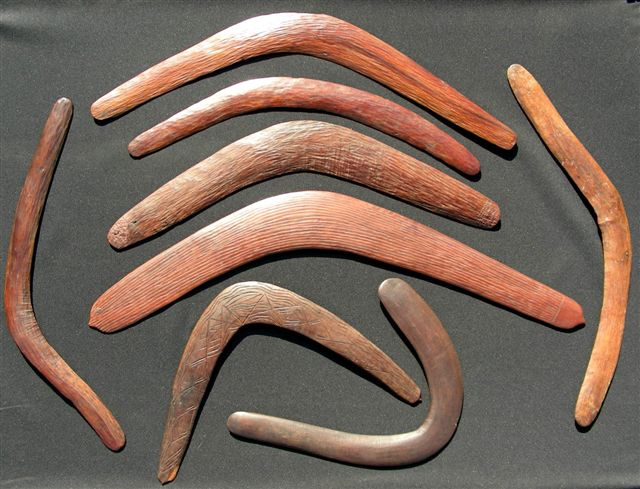
\includegraphics[scale=1]{imagenes/3-boomerang/boomerang_formas.jpg}
		\caption{Boomerangs de retorno.}
   	    \label{fig1}
		\end{center}
	\end{figure}


	Los boomerangs tradicionales son suavenmente convexos de un lado y casi planos del otro. Tienen alrededor de 6mm a 1 cm de grosor, de 5 a 7.5 cm de ancho, se extrecha hacía los extremos los cuales suelen estar redondeados ó punteados, el borde esta afilado por todas partes y la longitud varia desde 40 hasta 1 metro de longitud.

	\begin{figure}[h]
		\begin{center}
		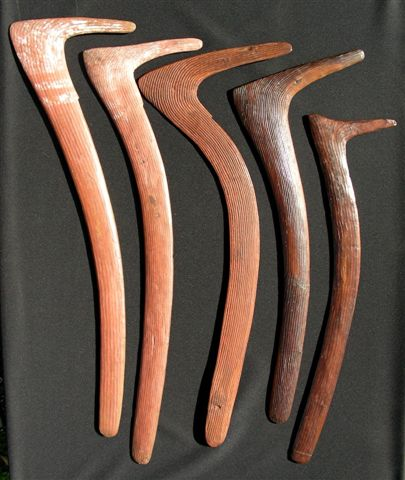
\includegraphics[scale=1]{imagenes/3-boomerang/boomerang_de_no_regreso.jpg}
		\caption{Boomerangs de no retorno.}
   	    \label{fig1}
		\end{center}
	\end{figure}

	Como se mencionó antes los boomerangs pueden ser de retorno y de no retorno, por lo que en este documento se estudian principalmente los de retorno, en particular, los llamados de 4 palas o en forma de cruz.

  \subsubsection*{Boomerangs de 4 palas}

  	Los boomerangs en forma de cruz están formadas for 4 palas de madera, las cuales tienen la misma forma que las palas de los boomerangs tradicionales.  Cada pala de tiene un tamaño de entre 20 y 30 cm de longitud y de 4 a 6 cm de ancho.

	Estos modelos también son llamados $"Cross Boomerangs"$ mostrados en la figura (\ref{fig1}), donde claramente puede notarse que difiere de los modelos tradicionales \cite{kuleshov}.
	\begin{figure}[h]
		\begin{center}
		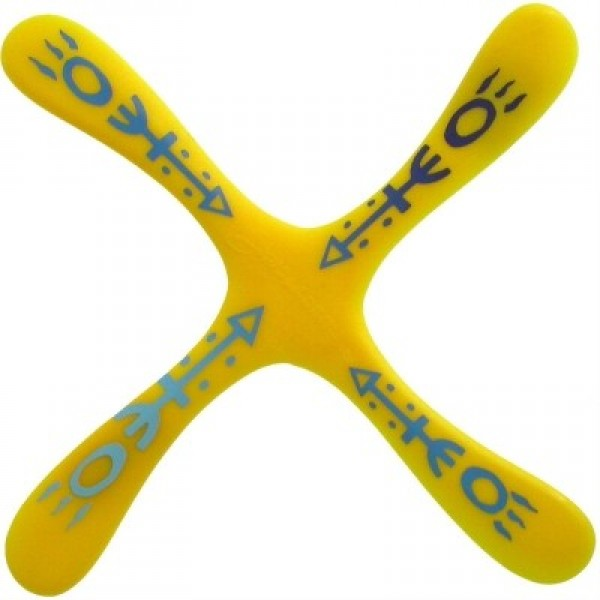
\includegraphics[scale=0.2]{imagenes/3-boomerang/boomerang4palas.jpg}
		\caption{Boomerang de 4 palas.}
   	    \label{fig1}
		\end{center}
	\end{figure}

	Para el análisis de los boomerang de 4 palas las ecuaciones de movimiento se siplifican considerablemente si consideramos que el centro de masa coincide con el punto de unión de las palas \cite{barger1973}.

	\subsection{Objetivos}

	\begin{enumerate}
	\item Modelo dinámico no lineal que describe la
	trayectoria tridimensional del boomerang en
	vuelo, a partir del lanzamiento inicial.

	\item Uso como soporte para la concepción de
	simulador computacional que describa la
	trayectoria tridimensional del boomerang.

	\item Captura de información paramétrica en vuelo
	mediante el uso de una Unidad de Medición
	Inercial miniaturizada embarcada: seguimiento de trayectoria en
	almacenamiento de datos y posterior despliegue en sistema informático.
	\end{enumerate}

	En el capítulo 1 se mostró una breve introducción sobre los boomerags, sus origenes y los objetivos generales a cubrir del proyecto. En el capítulo 2 se derivan las ecuaciones de movimiento del boomerang, así como las fuerzas que actúan sobre este y la consideración de la influencia del viento. En el capítulo 3 se presenta el simulador realizado para generar la trayectoria de vuelo del boomerang. En el capítulo 4 se presentan los experimentos y resultados obtenidos durante el desarrollo del proyecto.
